\section{Spark::Sp\-Window Class Reference}
\label{classSpark_1_1SpWindow}\index{Spark::SpWindow@{Spark::SpWindow}}
{\tt \#include $<$Sp\-Window.h$>$}

Collaboration diagram for Spark::Sp\-Window:\begin{figure}[H]
\begin{center}
\leavevmode
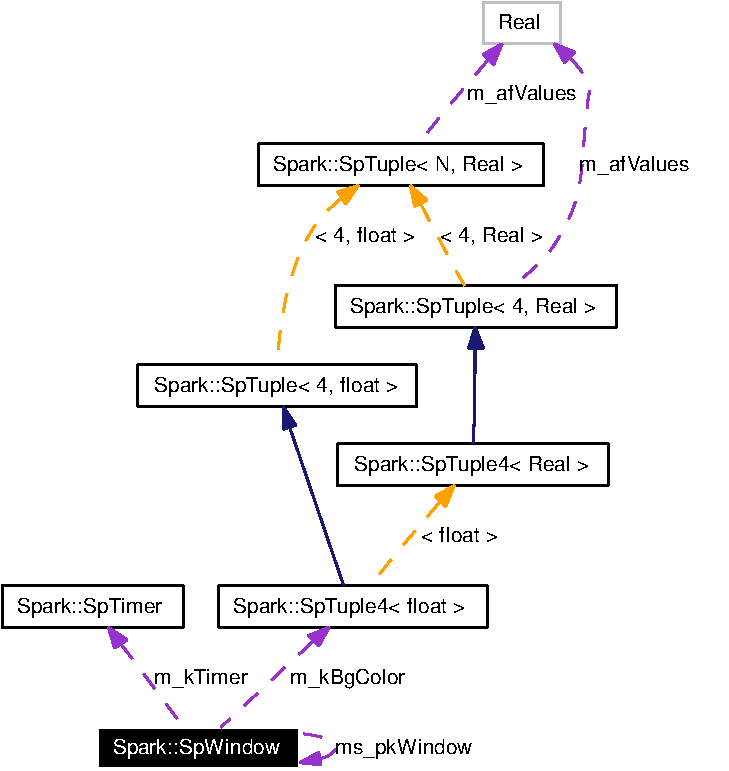
\includegraphics[width=192pt]{classSpark_1_1SpWindow__coll__graph}
\end{center}
\end{figure}


\subsection{Detailed Description}
Abstract base class for a graphical display window. 

Definition at line 37 of file Sp\-Window.h.\subsection*{Public Member Functions}
\begin{CompactItemize}
\item 
virtual {\bf $\sim$Sp\-Window} ()
\item 
virtual bool {\bf on\-Startup} ()
\item 
virtual bool {\bf on\-Initialize} ()
\item 
virtual void {\bf on\-Terminate} ()
\item 
virtual void {\bf on\-Move} (int i\-X, int i\-Y)
\item 
virtual void {\bf on\-Reshape} (int i\-Width, int i\-Height)
\item 
virtual void {\bf on\-Update} (int i\-Value)
\item 
virtual void {\bf on\-Display} ()
\item 
virtual void {\bf on\-Key\-Down} (unsigned char uc\-Key, int i\-X, int i\-Y)
\item 
virtual void {\bf on\-Key\-Up} (unsigned char uc\-Key, int i\-X, int i\-Y)
\item 
virtual void {\bf on\-Special\-Key\-Down} (int i\-Key, int i\-X, int i\-Y)
\item 
virtual void {\bf on\-Special\-Key\-Up} (int i\-Key, int i\-X, int i\-Y)
\item 
virtual void {\bf on\-Passive\-Motion} (int i\-X, int i\-Y)
\item 
virtual void {\bf on\-Mouse\-Motion} (int i\-X, int i\-Y, unsigned int ui\-Modifiers)
\item 
virtual void {\bf on\-Mouse\-Click} (int i\-Button, int i\-State, int i\-X, int i\-Y, unsigned int ui\-Modifiers)
\item 
virtual void {\bf on\-Idle} ()
\item 
void {\bf draw\-Image} (const unsigned char $\ast$auc\-Buffer, unsigned int ui\-Pos\-X, unsigned int ui\-Pos\-Y, unsigned int ui\-Width, unsigned int ui\-Height, bool b\-Alpha)
\item 
void {\bf draw\-Image} (const float $\ast$af\-Buffer, unsigned int ui\-Pos\-X, unsigned int ui\-Pos\-Y, unsigned int ui\-Width, unsigned int ui\-Height, bool b\-Alpha)
\item 
void {\bf draw\-String} (const char $\ast$pc\-String, int i\-X, int i\-Y, const {\bf Sp\-Color4f} \&rk\-Color)
\item 
void {\bf draw\-Frame\-Rate} (int i\-X, int i\-Y, const {\bf Sp\-Color4f} \&rk\-Color)
\item 
virtual void {\bf post\-Redisplay} ()
\item 
virtual void {\bf swap\-Buffers} ()
\item 
void {\bf update\-Clicks} ()
\item 
void {\bf make\-Current} ()
\item 
char $\ast$ {\bf title} ()
\item 
unsigned int {\bf x} ()
\item 
unsigned int {\bf y} ()
\item 
unsigned int {\bf width} ()
\item 
unsigned int {\bf height} ()
\item 
const {\bf Sp\-Color4f} \& {\bf bg} ()
\item 
{\bf Sp\-Timer} \& {\bf timer} ()
\item 
void {\bf set\-Window\-Id} (int i\-Sp\-Window\-ID)
\item 
int {\bf id} ()
\end{CompactItemize}
\subsection*{Static Public Member Functions}
\begin{CompactItemize}
\item 
{\bf Sp\-Window} $\ast$ {\bf current} ()
\end{CompactItemize}
\subsection*{Static Public Attributes}
\begin{CompactItemize}
\item 
const int {\bf KEY\_\-ESCAPE} = 0x1B
\item 
const int {\bf KEY\_\-LEFT\_\-ARROW} = GLUT\_\-KEY\_\-LEFT
\item 
const int {\bf KEY\_\-RIGHT\_\-ARROW} = GLUT\_\-KEY\_\-RIGHT
\item 
const int {\bf KEY\_\-UP\_\-ARROW} = GLUT\_\-KEY\_\-UP
\item 
const int {\bf KEY\_\-DOWN\_\-ARROW} = GLUT\_\-KEY\_\-DOWN
\item 
const int {\bf KEY\_\-HOME} = GLUT\_\-KEY\_\-HOME
\item 
const int {\bf KEY\_\-END} = GLUT\_\-KEY\_\-END
\item 
const int {\bf KEY\_\-PAGE\_\-UP} = GLUT\_\-KEY\_\-PAGE\_\-UP
\item 
const int {\bf KEY\_\-PAGE\_\-DOWN} = GLUT\_\-KEY\_\-PAGE\_\-DOWN
\item 
const int {\bf KEY\_\-INSERT} = GLUT\_\-KEY\_\-INSERT
\item 
const int {\bf KEY\_\-DELETE} = 0x2E
\item 
const int {\bf KEY\_\-F1} = GLUT\_\-KEY\_\-F1
\item 
const int {\bf KEY\_\-F2} = GLUT\_\-KEY\_\-F2
\item 
const int {\bf KEY\_\-F3} = GLUT\_\-KEY\_\-F3
\item 
const int {\bf KEY\_\-F4} = GLUT\_\-KEY\_\-F4
\item 
const int {\bf KEY\_\-F5} = GLUT\_\-KEY\_\-F5
\item 
const int {\bf KEY\_\-F6} = GLUT\_\-KEY\_\-F6
\item 
const int {\bf KEY\_\-F7} = GLUT\_\-KEY\_\-F7
\item 
const int {\bf KEY\_\-F8} = GLUT\_\-KEY\_\-F8
\item 
const int {\bf KEY\_\-F9} = GLUT\_\-KEY\_\-F9
\item 
const int {\bf KEY\_\-F10} = GLUT\_\-KEY\_\-F10
\item 
const int {\bf KEY\_\-F11} = GLUT\_\-KEY\_\-F11
\item 
const int {\bf KEY\_\-F12} = GLUT\_\-KEY\_\-F12
\item 
const int {\bf KEY\_\-SHIFT} = GLUT\_\-ACTIVE\_\-SHIFT
\item 
const int {\bf KEY\_\-CONTROL} = GLUT\_\-ACTIVE\_\-CTRL
\item 
const int {\bf KEY\_\-ALT} = GLUT\_\-ACTIVE\_\-ALT
\item 
const int {\bf KEY\_\-COMMAND} = 0
\item 
const int {\bf MOUSE\_\-LEFT\_\-BUTTON} = GLUT\_\-LEFT\_\-BUTTON
\item 
const int {\bf MOUSE\_\-MIDDLE\_\-BUTTON} = GLUT\_\-MIDDLE\_\-BUTTON
\item 
const int {\bf MOUSE\_\-RIGHT\_\-BUTTON} = GLUT\_\-RIGHT\_\-BUTTON
\item 
const int {\bf MOUSE\_\-UP} = GLUT\_\-UP
\item 
const int {\bf MOUSE\_\-DOWN} = GLUT\_\-DOWN
\item 
const int {\bf MOD\_\-LBUTTON}
\item 
const int {\bf MOD\_\-MBUTTON}
\item 
const int {\bf MOD\_\-RBUTTON}
\end{CompactItemize}
\subsection*{Protected Member Functions}
\begin{CompactItemize}
\item 
{\bf Sp\-Window} (char $\ast$ac\-Window\-Title, int i\-X, int i\-Y, int i\-Width, int i\-Height, const {\bf Sp\-Color4f} \&rk\-Bg\-Color)
\end{CompactItemize}
\subsection*{Protected Attributes}
\begin{CompactItemize}
\item 
bool {\bf m\_\-b\-Mouse\-Down}
\item 
bool {\bf m\_\-b\-Left\-Mouse\-Pressed}
\item 
bool {\bf m\_\-b\-Right\-Mouse\-Pressed}
\item 
bool {\bf m\_\-b\-Middle\-Mouse\-Pressed}
\item 
int {\bf m\_\-i\-Last\-Mouse\-X}
\item 
int {\bf m\_\-i\-Last\-Mouse\-Y}
\item 
float {\bf m\_\-f\-Frame\-Rate}
\item 
int {\bf m\_\-i\-Clicks}
\item 
int {\bf m\_\-i\-Timer}
\item 
int {\bf m\_\-i\-Max\-Timer}
\item 
char $\ast$ {\bf m\_\-ac\-Window\-Title}
\item 
int {\bf m\_\-i\-Sp\-Window\-ID}
\item 
int {\bf m\_\-i\-X}
\item 
int {\bf m\_\-i\-Y}
\item 
int {\bf m\_\-i\-Width}
\item 
int {\bf m\_\-i\-Height}
\item 
{\bf Sp\-Color4f} {\bf m\_\-k\-Bg\-Color}
\item 
{\bf Sp\-Timer} {\bf m\_\-k\-Timer}
\end{CompactItemize}
\subsection*{Static Protected Attributes}
\begin{CompactItemize}
\item 
{\bf Sp\-Window} $\ast$ {\bf ms\_\-pk\-Window} = NULL
\end{CompactItemize}


\subsection{Constructor \& Destructor Documentation}
\index{Spark::SpWindow@{Spark::Sp\-Window}!~SpWindow@{$\sim$SpWindow}}
\index{~SpWindow@{$\sim$SpWindow}!Spark::SpWindow@{Spark::Sp\-Window}}
\subsubsection{\setlength{\rightskip}{0pt plus 5cm}Sp\-Window::$\sim${\bf Sp\-Window} ()\hspace{0.3cm}{\tt  [virtual]}}\label{classSpark_1_1SpWindow_a0}


Definition at line 25 of file Sp\-Window.cpp.

References ms\_\-pk\-Window, and on\-Terminate().\index{Spark::SpWindow@{Spark::Sp\-Window}!SpWindow@{SpWindow}}
\index{SpWindow@{SpWindow}!Spark::SpWindow@{Spark::Sp\-Window}}
\subsubsection{\setlength{\rightskip}{0pt plus 5cm}Sp\-Window::Sp\-Window (char $\ast$ {\em ac\-Window\-Title}, int {\em i\-X}, int {\em i\-Y}, int {\em i\-Width}, int {\em i\-Height}, const {\bf Sp\-Color4f} \& {\em rk\-Bg\-Color})\hspace{0.3cm}{\tt  [protected]}}\label{classSpark_1_1SpWindow_b0}


Definition at line 9 of file Sp\-Window.cpp.

References m\_\-ac\-Window\-Title, m\_\-i\-Clicks, m\_\-i\-Height, m\_\-i\-Max\-Timer, m\_\-i\-Timer, m\_\-i\-Width, m\_\-i\-X, m\_\-i\-Y, m\_\-k\-Bg\-Color, ms\_\-pk\-Window, and Spark::Sp\-Color4f.

\subsection{Member Function Documentation}
\index{Spark::SpWindow@{Spark::Sp\-Window}!bg@{bg}}
\index{bg@{bg}!Spark::SpWindow@{Spark::Sp\-Window}}
\subsubsection{\setlength{\rightskip}{0pt plus 5cm}const {\bf Sp\-Color4f} \& Spark::Sp\-Window::bg ()\hspace{0.3cm}{\tt  [inline]}}\label{classSpark_1_1SpWindow_a29}


Definition at line 235 of file Sp\-Window.h.\index{Spark::SpWindow@{Spark::Sp\-Window}!current@{current}}
\index{current@{current}!Spark::SpWindow@{Spark::Sp\-Window}}
\subsubsection{\setlength{\rightskip}{0pt plus 5cm}{\bf Sp\-Window} $\ast$ Spark::Sp\-Window::current ()\hspace{0.3cm}{\tt  [inline, static]}}\label{classSpark_1_1SpWindow_e0}


Definition at line 205 of file Sp\-Window.h.

Referenced by main().\index{Spark::SpWindow@{Spark::Sp\-Window}!drawFrameRate@{drawFrameRate}}
\index{drawFrameRate@{drawFrameRate}!Spark::SpWindow@{Spark::Sp\-Window}}
\subsubsection{\setlength{\rightskip}{0pt plus 5cm}void Sp\-Window::draw\-Frame\-Rate (int {\em i\-X}, int {\em i\-Y}, const {\bf Sp\-Color4f} \& {\em rk\-Color})}\label{classSpark_1_1SpWindow_a19}


Definition at line 132 of file Sp\-Window.cpp.

References draw\-String(), Spark::Sp\-Timer::elapsed\-Seconds(), m\_\-f\-Frame\-Rate, m\_\-i\-Clicks, m\_\-i\-Max\-Timer, m\_\-i\-Timer, m\_\-k\-Timer, and Spark::Sp\-Color4f.\index{Spark::SpWindow@{Spark::Sp\-Window}!drawImage@{drawImage}}
\index{drawImage@{drawImage}!Spark::SpWindow@{Spark::Sp\-Window}}
\subsubsection{\setlength{\rightskip}{0pt plus 5cm}void Sp\-Window::draw\-Image (const float $\ast$ {\em af\-Buffer}, unsigned int {\em ui\-Pos\-X}, unsigned int {\em ui\-Pos\-Y}, unsigned int {\em ui\-Width}, unsigned int {\em ui\-Height}, bool {\em b\-Alpha})}\label{classSpark_1_1SpWindow_a17}


Definition at line 210 of file Sp\-Glut\-Window.cpp.

References m\_\-i\-Height, and m\_\-i\-Width.\index{Spark::SpWindow@{Spark::Sp\-Window}!drawImage@{drawImage}}
\index{drawImage@{drawImage}!Spark::SpWindow@{Spark::Sp\-Window}}
\subsubsection{\setlength{\rightskip}{0pt plus 5cm}void Sp\-Window::draw\-Image (const unsigned char $\ast$ {\em auc\-Buffer}, unsigned int {\em ui\-Pos\-X}, unsigned int {\em ui\-Pos\-Y}, unsigned int {\em ui\-Width}, unsigned int {\em ui\-Height}, bool {\em b\-Alpha})}\label{classSpark_1_1SpWindow_a16}


Definition at line 148 of file Sp\-Glut\-Window.cpp.

References m\_\-i\-Height, and m\_\-i\-Width.\index{Spark::SpWindow@{Spark::Sp\-Window}!drawString@{drawString}}
\index{drawString@{drawString}!Spark::SpWindow@{Spark::Sp\-Window}}
\subsubsection{\setlength{\rightskip}{0pt plus 5cm}void Sp\-Window::draw\-String (const char $\ast$ {\em pc\-String}, int {\em i\-X}, int {\em i\-Y}, const {\bf Sp\-Color4f} \& {\em rk\-Color})}\label{classSpark_1_1SpWindow_a18}


Definition at line 132 of file Sp\-Glut\-Window.cpp.

References Spark::Sp\-Tuple4$<$ Real $>$::a(), Spark::Sp\-Tuple4$<$ Real $>$::b(), Spark::Sp\-Tuple4$<$ Real $>$::g(), Spark::Sp\-Tuple4$<$ Real $>$::r(), and Spark::Sp\-Color4f.

Referenced by draw\-Frame\-Rate().\index{Spark::SpWindow@{Spark::Sp\-Window}!height@{height}}
\index{height@{height}!Spark::SpWindow@{Spark::Sp\-Window}}
\subsubsection{\setlength{\rightskip}{0pt plus 5cm}unsigned int Spark::Sp\-Window::height ()\hspace{0.3cm}{\tt  [inline]}}\label{classSpark_1_1SpWindow_a28}


Definition at line 230 of file Sp\-Window.h.

Referenced by main().\index{Spark::SpWindow@{Spark::Sp\-Window}!id@{id}}
\index{id@{id}!Spark::SpWindow@{Spark::Sp\-Window}}
\subsubsection{\setlength{\rightskip}{0pt plus 5cm}int Spark::Sp\-Window::id ()\hspace{0.3cm}{\tt  [inline]}}\label{classSpark_1_1SpWindow_a32}


Definition at line 245 of file Sp\-Window.h.

Referenced by main().\index{Spark::SpWindow@{Spark::Sp\-Window}!makeCurrent@{makeCurrent}}
\index{makeCurrent@{makeCurrent}!Spark::SpWindow@{Spark::Sp\-Window}}
\subsubsection{\setlength{\rightskip}{0pt plus 5cm}void Sp\-Window::make\-Current ()}\label{classSpark_1_1SpWindow_a23}


Definition at line 116 of file Sp\-Glut\-Window.cpp.

References ms\_\-pk\-Window.\index{Spark::SpWindow@{Spark::Sp\-Window}!onDisplay@{onDisplay}}
\index{onDisplay@{onDisplay}!Spark::SpWindow@{Spark::Sp\-Window}}
\subsubsection{\setlength{\rightskip}{0pt plus 5cm}void Sp\-Window::on\-Display ()\hspace{0.3cm}{\tt  [virtual]}}\label{classSpark_1_1SpWindow_a7}


Definition at line 54 of file Sp\-Window.cpp.\index{Spark::SpWindow@{Spark::Sp\-Window}!onIdle@{onIdle}}
\index{onIdle@{onIdle}!Spark::SpWindow@{Spark::Sp\-Window}}
\subsubsection{\setlength{\rightskip}{0pt plus 5cm}void Sp\-Window::on\-Idle ()\hspace{0.3cm}{\tt  [virtual]}}\label{classSpark_1_1SpWindow_a15}


Definition at line 59 of file Sp\-Window.cpp.

References Spark::Sp\-Timer::elapsed\-Count(), m\_\-k\-Timer, on\-Update(), and post\-Redisplay().\index{Spark::SpWindow@{Spark::Sp\-Window}!onInitialize@{onInitialize}}
\index{onInitialize@{onInitialize}!Spark::SpWindow@{Spark::Sp\-Window}}
\subsubsection{\setlength{\rightskip}{0pt plus 5cm}bool Sp\-Window::on\-Initialize ()\hspace{0.3cm}{\tt  [virtual]}}\label{classSpark_1_1SpWindow_a2}


Definition at line 37 of file Sp\-Window.cpp.

Referenced by main().\index{Spark::SpWindow@{Spark::Sp\-Window}!onKeyDown@{onKeyDown}}
\index{onKeyDown@{onKeyDown}!Spark::SpWindow@{Spark::Sp\-Window}}
\subsubsection{\setlength{\rightskip}{0pt plus 5cm}void Sp\-Window::on\-Key\-Down (unsigned char {\em uc\-Key}, int {\em i\-X}, int {\em i\-Y})\hspace{0.3cm}{\tt  [virtual]}}\label{classSpark_1_1SpWindow_a8}


Definition at line 65 of file Sp\-Window.cpp.

References KEY\_\-ESCAPE, and on\-Terminate().\index{Spark::SpWindow@{Spark::Sp\-Window}!onKeyUp@{onKeyUp}}
\index{onKeyUp@{onKeyUp}!Spark::SpWindow@{Spark::Sp\-Window}}
\subsubsection{\setlength{\rightskip}{0pt plus 5cm}void Sp\-Window::on\-Key\-Up (unsigned char {\em uc\-Key}, int {\em i\-X}, int {\em i\-Y})\hspace{0.3cm}{\tt  [virtual]}}\label{classSpark_1_1SpWindow_a9}


Definition at line 72 of file Sp\-Window.cpp.\index{Spark::SpWindow@{Spark::Sp\-Window}!onMouseClick@{onMouseClick}}
\index{onMouseClick@{onMouseClick}!Spark::SpWindow@{Spark::Sp\-Window}}
\subsubsection{\setlength{\rightskip}{0pt plus 5cm}void Sp\-Window::on\-Mouse\-Click (int {\em i\-Button}, int {\em i\-State}, int {\em i\-X}, int {\em i\-Y}, unsigned int {\em ui\-Modifiers})\hspace{0.3cm}{\tt  [virtual]}}\label{classSpark_1_1SpWindow_a14}


Definition at line 87 of file Sp\-Window.cpp.

References m\_\-b\-Left\-Mouse\-Pressed, m\_\-b\-Middle\-Mouse\-Pressed, m\_\-b\-Mouse\-Down, m\_\-b\-Right\-Mouse\-Pressed, m\_\-i\-Last\-Mouse\-X, and m\_\-i\-Last\-Mouse\-Y.\index{Spark::SpWindow@{Spark::Sp\-Window}!onMouseMotion@{onMouseMotion}}
\index{onMouseMotion@{onMouseMotion}!Spark::SpWindow@{Spark::Sp\-Window}}
\subsubsection{\setlength{\rightskip}{0pt plus 5cm}void Sp\-Window::on\-Mouse\-Motion (int {\em i\-X}, int {\em i\-Y}, unsigned int {\em ui\-Modifiers})\hspace{0.3cm}{\tt  [virtual]}}\label{classSpark_1_1SpWindow_a13}


Definition at line 115 of file Sp\-Window.cpp.\index{Spark::SpWindow@{Spark::Sp\-Window}!onMove@{onMove}}
\index{onMove@{onMove}!Spark::SpWindow@{Spark::Sp\-Window}}
\subsubsection{\setlength{\rightskip}{0pt plus 5cm}void Sp\-Window::on\-Move (int {\em i\-X}, int {\em i\-Y})\hspace{0.3cm}{\tt  [virtual]}}\label{classSpark_1_1SpWindow_a4}


Definition at line 42 of file Sp\-Window.cpp.

References m\_\-i\-X, and m\_\-i\-Y.\index{Spark::SpWindow@{Spark::Sp\-Window}!onPassiveMotion@{onPassiveMotion}}
\index{onPassiveMotion@{onPassiveMotion}!Spark::SpWindow@{Spark::Sp\-Window}}
\subsubsection{\setlength{\rightskip}{0pt plus 5cm}void Sp\-Window::on\-Passive\-Motion (int {\em i\-X}, int {\em i\-Y})\hspace{0.3cm}{\tt  [virtual]}}\label{classSpark_1_1SpWindow_a12}


Definition at line 120 of file Sp\-Window.cpp.\index{Spark::SpWindow@{Spark::Sp\-Window}!onReshape@{onReshape}}
\index{onReshape@{onReshape}!Spark::SpWindow@{Spark::Sp\-Window}}
\subsubsection{\setlength{\rightskip}{0pt plus 5cm}void Sp\-Window::on\-Reshape (int {\em i\-Width}, int {\em i\-Height})\hspace{0.3cm}{\tt  [virtual]}}\label{classSpark_1_1SpWindow_a5}


Definition at line 48 of file Sp\-Window.cpp.

References m\_\-i\-Height, and m\_\-i\-Width.\index{Spark::SpWindow@{Spark::Sp\-Window}!onSpecialKeyDown@{onSpecialKeyDown}}
\index{onSpecialKeyDown@{onSpecialKeyDown}!Spark::SpWindow@{Spark::Sp\-Window}}
\subsubsection{\setlength{\rightskip}{0pt plus 5cm}void Sp\-Window::on\-Special\-Key\-Down (int {\em i\-Key}, int {\em i\-X}, int {\em i\-Y})\hspace{0.3cm}{\tt  [virtual]}}\label{classSpark_1_1SpWindow_a10}


Definition at line 77 of file Sp\-Window.cpp.\index{Spark::SpWindow@{Spark::Sp\-Window}!onSpecialKeyUp@{onSpecialKeyUp}}
\index{onSpecialKeyUp@{onSpecialKeyUp}!Spark::SpWindow@{Spark::Sp\-Window}}
\subsubsection{\setlength{\rightskip}{0pt plus 5cm}void Sp\-Window::on\-Special\-Key\-Up (int {\em i\-Key}, int {\em i\-X}, int {\em i\-Y})\hspace{0.3cm}{\tt  [virtual]}}\label{classSpark_1_1SpWindow_a11}


Definition at line 82 of file Sp\-Window.cpp.\index{Spark::SpWindow@{Spark::Sp\-Window}!onStartup@{onStartup}}
\index{onStartup@{onStartup}!Spark::SpWindow@{Spark::Sp\-Window}}
\subsubsection{\setlength{\rightskip}{0pt plus 5cm}bool Sp\-Window::on\-Startup ()\hspace{0.3cm}{\tt  [virtual]}}\label{classSpark_1_1SpWindow_a1}


Definition at line 32 of file Sp\-Window.cpp.

Referenced by main().\index{Spark::SpWindow@{Spark::Sp\-Window}!onTerminate@{onTerminate}}
\index{onTerminate@{onTerminate}!Spark::SpWindow@{Spark::Sp\-Window}}
\subsubsection{\setlength{\rightskip}{0pt plus 5cm}void Sp\-Window::on\-Terminate ()\hspace{0.3cm}{\tt  [virtual]}}\label{classSpark_1_1SpWindow_a3}


Definition at line 102 of file Sp\-Glut\-Window.cpp.

Referenced by on\-Key\-Down(), and $\sim$Sp\-Window().\index{Spark::SpWindow@{Spark::Sp\-Window}!onUpdate@{onUpdate}}
\index{onUpdate@{onUpdate}!Spark::SpWindow@{Spark::Sp\-Window}}
\subsubsection{\setlength{\rightskip}{0pt plus 5cm}void Sp\-Window::on\-Update (int {\em i\-Value})\hspace{0.3cm}{\tt  [virtual]}}\label{classSpark_1_1SpWindow_a6}


Definition at line 107 of file Sp\-Glut\-Window.cpp.

References post\-Redisplay().

Referenced by on\-Idle().\index{Spark::SpWindow@{Spark::Sp\-Window}!postRedisplay@{postRedisplay}}
\index{postRedisplay@{postRedisplay}!Spark::SpWindow@{Spark::Sp\-Window}}
\subsubsection{\setlength{\rightskip}{0pt plus 5cm}void Sp\-Window::post\-Redisplay ()\hspace{0.3cm}{\tt  [virtual]}}\label{classSpark_1_1SpWindow_a20}


Definition at line 122 of file Sp\-Glut\-Window.cpp.

Referenced by on\-Idle(), and on\-Update().\index{Spark::SpWindow@{Spark::Sp\-Window}!setWindowId@{setWindowId}}
\index{setWindowId@{setWindowId}!Spark::SpWindow@{Spark::Sp\-Window}}
\subsubsection{\setlength{\rightskip}{0pt plus 5cm}void Spark::Sp\-Window::set\-Window\-Id (int {\em i\-Sp\-Window\-ID})\hspace{0.3cm}{\tt  [inline]}}\label{classSpark_1_1SpWindow_a31}


Definition at line 240 of file Sp\-Window.h.

Referenced by main().\index{Spark::SpWindow@{Spark::Sp\-Window}!swapBuffers@{swapBuffers}}
\index{swapBuffers@{swapBuffers}!Spark::SpWindow@{Spark::Sp\-Window}}
\subsubsection{\setlength{\rightskip}{0pt plus 5cm}void Sp\-Window::swap\-Buffers ()\hspace{0.3cm}{\tt  [virtual]}}\label{classSpark_1_1SpWindow_a21}


Definition at line 127 of file Sp\-Glut\-Window.cpp.\index{Spark::SpWindow@{Spark::Sp\-Window}!timer@{timer}}
\index{timer@{timer}!Spark::SpWindow@{Spark::Sp\-Window}}
\subsubsection{\setlength{\rightskip}{0pt plus 5cm}{\bf Sp\-Timer} \& Spark::Sp\-Window::timer ()\hspace{0.3cm}{\tt  [inline]}}\label{classSpark_1_1SpWindow_a30}


Definition at line 250 of file Sp\-Window.h.\index{Spark::SpWindow@{Spark::Sp\-Window}!title@{title}}
\index{title@{title}!Spark::SpWindow@{Spark::Sp\-Window}}
\subsubsection{\setlength{\rightskip}{0pt plus 5cm}char $\ast$ Spark::Sp\-Window::title ()\hspace{0.3cm}{\tt  [inline]}}\label{classSpark_1_1SpWindow_a24}


Definition at line 210 of file Sp\-Window.h.

Referenced by main().\index{Spark::SpWindow@{Spark::Sp\-Window}!updateClicks@{updateClicks}}
\index{updateClicks@{updateClicks}!Spark::SpWindow@{Spark::Sp\-Window}}
\subsubsection{\setlength{\rightskip}{0pt plus 5cm}void Sp\-Window::update\-Clicks ()}\label{classSpark_1_1SpWindow_a22}


Definition at line 125 of file Sp\-Window.cpp.

References m\_\-i\-Clicks.\index{Spark::SpWindow@{Spark::Sp\-Window}!width@{width}}
\index{width@{width}!Spark::SpWindow@{Spark::Sp\-Window}}
\subsubsection{\setlength{\rightskip}{0pt plus 5cm}unsigned int Spark::Sp\-Window::width ()\hspace{0.3cm}{\tt  [inline]}}\label{classSpark_1_1SpWindow_a27}


Definition at line 225 of file Sp\-Window.h.

Referenced by main().\index{Spark::SpWindow@{Spark::Sp\-Window}!x@{x}}
\index{x@{x}!Spark::SpWindow@{Spark::Sp\-Window}}
\subsubsection{\setlength{\rightskip}{0pt plus 5cm}unsigned int Spark::Sp\-Window::x ()\hspace{0.3cm}{\tt  [inline]}}\label{classSpark_1_1SpWindow_a25}


Definition at line 215 of file Sp\-Window.h.\index{Spark::SpWindow@{Spark::Sp\-Window}!y@{y}}
\index{y@{y}!Spark::SpWindow@{Spark::Sp\-Window}}
\subsubsection{\setlength{\rightskip}{0pt plus 5cm}unsigned int Spark::Sp\-Window::y ()\hspace{0.3cm}{\tt  [inline]}}\label{classSpark_1_1SpWindow_a26}


Definition at line 220 of file Sp\-Window.h.

\subsection{Member Data Documentation}
\index{Spark::SpWindow@{Spark::Sp\-Window}!KEY_ALT@{KEY\_\-ALT}}
\index{KEY_ALT@{KEY\_\-ALT}!Spark::SpWindow@{Spark::Sp\-Window}}
\subsubsection{\setlength{\rightskip}{0pt plus 5cm}const int {\bf Sp\-Window::KEY\_\-ALT} = GLUT\_\-ACTIVE\_\-ALT\hspace{0.3cm}{\tt  [static]}}\label{classSpark_1_1SpWindow_s25}


Definition at line 59 of file Sp\-Glut\-Key\-Bindings.h.\index{Spark::SpWindow@{Spark::Sp\-Window}!KEY_COMMAND@{KEY\_\-COMMAND}}
\index{KEY_COMMAND@{KEY\_\-COMMAND}!Spark::SpWindow@{Spark::Sp\-Window}}
\subsubsection{\setlength{\rightskip}{0pt plus 5cm}const int {\bf Sp\-Window::KEY\_\-COMMAND} = 0\hspace{0.3cm}{\tt  [static]}}\label{classSpark_1_1SpWindow_s26}


Definition at line 60 of file Sp\-Glut\-Key\-Bindings.h.\index{Spark::SpWindow@{Spark::Sp\-Window}!KEY_CONTROL@{KEY\_\-CONTROL}}
\index{KEY_CONTROL@{KEY\_\-CONTROL}!Spark::SpWindow@{Spark::Sp\-Window}}
\subsubsection{\setlength{\rightskip}{0pt plus 5cm}const int {\bf Sp\-Window::KEY\_\-CONTROL} = GLUT\_\-ACTIVE\_\-CTRL\hspace{0.3cm}{\tt  [static]}}\label{classSpark_1_1SpWindow_s24}


Definition at line 58 of file Sp\-Glut\-Key\-Bindings.h.\index{Spark::SpWindow@{Spark::Sp\-Window}!KEY_DELETE@{KEY\_\-DELETE}}
\index{KEY_DELETE@{KEY\_\-DELETE}!Spark::SpWindow@{Spark::Sp\-Window}}
\subsubsection{\setlength{\rightskip}{0pt plus 5cm}const int {\bf Sp\-Window::KEY\_\-DELETE} = 0x2E\hspace{0.3cm}{\tt  [static]}}\label{classSpark_1_1SpWindow_s10}


Definition at line 41 of file Sp\-Glut\-Key\-Bindings.h.\index{Spark::SpWindow@{Spark::Sp\-Window}!KEY_DOWN_ARROW@{KEY\_\-DOWN\_\-ARROW}}
\index{KEY_DOWN_ARROW@{KEY\_\-DOWN\_\-ARROW}!Spark::SpWindow@{Spark::Sp\-Window}}
\subsubsection{\setlength{\rightskip}{0pt plus 5cm}const int {\bf Sp\-Window::KEY\_\-DOWN\_\-ARROW} = GLUT\_\-KEY\_\-DOWN\hspace{0.3cm}{\tt  [static]}}\label{classSpark_1_1SpWindow_s4}


Definition at line 35 of file Sp\-Glut\-Key\-Bindings.h.\index{Spark::SpWindow@{Spark::Sp\-Window}!KEY_END@{KEY\_\-END}}
\index{KEY_END@{KEY\_\-END}!Spark::SpWindow@{Spark::Sp\-Window}}
\subsubsection{\setlength{\rightskip}{0pt plus 5cm}const int {\bf Sp\-Window::KEY\_\-END} = GLUT\_\-KEY\_\-END\hspace{0.3cm}{\tt  [static]}}\label{classSpark_1_1SpWindow_s6}


Definition at line 37 of file Sp\-Glut\-Key\-Bindings.h.\index{Spark::SpWindow@{Spark::Sp\-Window}!KEY_ESCAPE@{KEY\_\-ESCAPE}}
\index{KEY_ESCAPE@{KEY\_\-ESCAPE}!Spark::SpWindow@{Spark::Sp\-Window}}
\subsubsection{\setlength{\rightskip}{0pt plus 5cm}const int {\bf Sp\-Window::KEY\_\-ESCAPE} = 0x1B\hspace{0.3cm}{\tt  [static]}}\label{classSpark_1_1SpWindow_s0}


Definition at line 31 of file Sp\-Glut\-Key\-Bindings.h.

Referenced by on\-Key\-Down().\index{Spark::SpWindow@{Spark::Sp\-Window}!KEY_F1@{KEY\_\-F1}}
\index{KEY_F1@{KEY\_\-F1}!Spark::SpWindow@{Spark::Sp\-Window}}
\subsubsection{\setlength{\rightskip}{0pt plus 5cm}const int {\bf Sp\-Window::KEY\_\-F1} = GLUT\_\-KEY\_\-F1\hspace{0.3cm}{\tt  [static]}}\label{classSpark_1_1SpWindow_s11}


Definition at line 42 of file Sp\-Glut\-Key\-Bindings.h.\index{Spark::SpWindow@{Spark::Sp\-Window}!KEY_F10@{KEY\_\-F10}}
\index{KEY_F10@{KEY\_\-F10}!Spark::SpWindow@{Spark::Sp\-Window}}
\subsubsection{\setlength{\rightskip}{0pt plus 5cm}const int {\bf Sp\-Window::KEY\_\-F10} = GLUT\_\-KEY\_\-F10\hspace{0.3cm}{\tt  [static]}}\label{classSpark_1_1SpWindow_s20}


Definition at line 51 of file Sp\-Glut\-Key\-Bindings.h.\index{Spark::SpWindow@{Spark::Sp\-Window}!KEY_F11@{KEY\_\-F11}}
\index{KEY_F11@{KEY\_\-F11}!Spark::SpWindow@{Spark::Sp\-Window}}
\subsubsection{\setlength{\rightskip}{0pt plus 5cm}const int {\bf Sp\-Window::KEY\_\-F11} = GLUT\_\-KEY\_\-F11\hspace{0.3cm}{\tt  [static]}}\label{classSpark_1_1SpWindow_s21}


Definition at line 52 of file Sp\-Glut\-Key\-Bindings.h.\index{Spark::SpWindow@{Spark::Sp\-Window}!KEY_F12@{KEY\_\-F12}}
\index{KEY_F12@{KEY\_\-F12}!Spark::SpWindow@{Spark::Sp\-Window}}
\subsubsection{\setlength{\rightskip}{0pt plus 5cm}const int {\bf Sp\-Window::KEY\_\-F12} = GLUT\_\-KEY\_\-F12\hspace{0.3cm}{\tt  [static]}}\label{classSpark_1_1SpWindow_s22}


Definition at line 53 of file Sp\-Glut\-Key\-Bindings.h.\index{Spark::SpWindow@{Spark::Sp\-Window}!KEY_F2@{KEY\_\-F2}}
\index{KEY_F2@{KEY\_\-F2}!Spark::SpWindow@{Spark::Sp\-Window}}
\subsubsection{\setlength{\rightskip}{0pt plus 5cm}const int {\bf Sp\-Window::KEY\_\-F2} = GLUT\_\-KEY\_\-F2\hspace{0.3cm}{\tt  [static]}}\label{classSpark_1_1SpWindow_s12}


Definition at line 43 of file Sp\-Glut\-Key\-Bindings.h.\index{Spark::SpWindow@{Spark::Sp\-Window}!KEY_F3@{KEY\_\-F3}}
\index{KEY_F3@{KEY\_\-F3}!Spark::SpWindow@{Spark::Sp\-Window}}
\subsubsection{\setlength{\rightskip}{0pt plus 5cm}const int {\bf Sp\-Window::KEY\_\-F3} = GLUT\_\-KEY\_\-F3\hspace{0.3cm}{\tt  [static]}}\label{classSpark_1_1SpWindow_s13}


Definition at line 44 of file Sp\-Glut\-Key\-Bindings.h.\index{Spark::SpWindow@{Spark::Sp\-Window}!KEY_F4@{KEY\_\-F4}}
\index{KEY_F4@{KEY\_\-F4}!Spark::SpWindow@{Spark::Sp\-Window}}
\subsubsection{\setlength{\rightskip}{0pt plus 5cm}const int {\bf Sp\-Window::KEY\_\-F4} = GLUT\_\-KEY\_\-F4\hspace{0.3cm}{\tt  [static]}}\label{classSpark_1_1SpWindow_s14}


Definition at line 45 of file Sp\-Glut\-Key\-Bindings.h.\index{Spark::SpWindow@{Spark::Sp\-Window}!KEY_F5@{KEY\_\-F5}}
\index{KEY_F5@{KEY\_\-F5}!Spark::SpWindow@{Spark::Sp\-Window}}
\subsubsection{\setlength{\rightskip}{0pt plus 5cm}const int {\bf Sp\-Window::KEY\_\-F5} = GLUT\_\-KEY\_\-F5\hspace{0.3cm}{\tt  [static]}}\label{classSpark_1_1SpWindow_s15}


Definition at line 46 of file Sp\-Glut\-Key\-Bindings.h.\index{Spark::SpWindow@{Spark::Sp\-Window}!KEY_F6@{KEY\_\-F6}}
\index{KEY_F6@{KEY\_\-F6}!Spark::SpWindow@{Spark::Sp\-Window}}
\subsubsection{\setlength{\rightskip}{0pt plus 5cm}const int {\bf Sp\-Window::KEY\_\-F6} = GLUT\_\-KEY\_\-F6\hspace{0.3cm}{\tt  [static]}}\label{classSpark_1_1SpWindow_s16}


Definition at line 47 of file Sp\-Glut\-Key\-Bindings.h.\index{Spark::SpWindow@{Spark::Sp\-Window}!KEY_F7@{KEY\_\-F7}}
\index{KEY_F7@{KEY\_\-F7}!Spark::SpWindow@{Spark::Sp\-Window}}
\subsubsection{\setlength{\rightskip}{0pt plus 5cm}const int {\bf Sp\-Window::KEY\_\-F7} = GLUT\_\-KEY\_\-F7\hspace{0.3cm}{\tt  [static]}}\label{classSpark_1_1SpWindow_s17}


Definition at line 48 of file Sp\-Glut\-Key\-Bindings.h.\index{Spark::SpWindow@{Spark::Sp\-Window}!KEY_F8@{KEY\_\-F8}}
\index{KEY_F8@{KEY\_\-F8}!Spark::SpWindow@{Spark::Sp\-Window}}
\subsubsection{\setlength{\rightskip}{0pt plus 5cm}const int {\bf Sp\-Window::KEY\_\-F8} = GLUT\_\-KEY\_\-F8\hspace{0.3cm}{\tt  [static]}}\label{classSpark_1_1SpWindow_s18}


Definition at line 49 of file Sp\-Glut\-Key\-Bindings.h.\index{Spark::SpWindow@{Spark::Sp\-Window}!KEY_F9@{KEY\_\-F9}}
\index{KEY_F9@{KEY\_\-F9}!Spark::SpWindow@{Spark::Sp\-Window}}
\subsubsection{\setlength{\rightskip}{0pt plus 5cm}const int {\bf Sp\-Window::KEY\_\-F9} = GLUT\_\-KEY\_\-F9\hspace{0.3cm}{\tt  [static]}}\label{classSpark_1_1SpWindow_s19}


Definition at line 50 of file Sp\-Glut\-Key\-Bindings.h.\index{Spark::SpWindow@{Spark::Sp\-Window}!KEY_HOME@{KEY\_\-HOME}}
\index{KEY_HOME@{KEY\_\-HOME}!Spark::SpWindow@{Spark::Sp\-Window}}
\subsubsection{\setlength{\rightskip}{0pt plus 5cm}const int {\bf Sp\-Window::KEY\_\-HOME} = GLUT\_\-KEY\_\-HOME\hspace{0.3cm}{\tt  [static]}}\label{classSpark_1_1SpWindow_s5}


Definition at line 36 of file Sp\-Glut\-Key\-Bindings.h.\index{Spark::SpWindow@{Spark::Sp\-Window}!KEY_INSERT@{KEY\_\-INSERT}}
\index{KEY_INSERT@{KEY\_\-INSERT}!Spark::SpWindow@{Spark::Sp\-Window}}
\subsubsection{\setlength{\rightskip}{0pt plus 5cm}const int {\bf Sp\-Window::KEY\_\-INSERT} = GLUT\_\-KEY\_\-INSERT\hspace{0.3cm}{\tt  [static]}}\label{classSpark_1_1SpWindow_s9}


Definition at line 40 of file Sp\-Glut\-Key\-Bindings.h.\index{Spark::SpWindow@{Spark::Sp\-Window}!KEY_LEFT_ARROW@{KEY\_\-LEFT\_\-ARROW}}
\index{KEY_LEFT_ARROW@{KEY\_\-LEFT\_\-ARROW}!Spark::SpWindow@{Spark::Sp\-Window}}
\subsubsection{\setlength{\rightskip}{0pt plus 5cm}const int {\bf Sp\-Window::KEY\_\-LEFT\_\-ARROW} = GLUT\_\-KEY\_\-LEFT\hspace{0.3cm}{\tt  [static]}}\label{classSpark_1_1SpWindow_s1}


Definition at line 32 of file Sp\-Glut\-Key\-Bindings.h.\index{Spark::SpWindow@{Spark::Sp\-Window}!KEY_PAGE_DOWN@{KEY\_\-PAGE\_\-DOWN}}
\index{KEY_PAGE_DOWN@{KEY\_\-PAGE\_\-DOWN}!Spark::SpWindow@{Spark::Sp\-Window}}
\subsubsection{\setlength{\rightskip}{0pt plus 5cm}const int {\bf Sp\-Window::KEY\_\-PAGE\_\-DOWN} = GLUT\_\-KEY\_\-PAGE\_\-DOWN\hspace{0.3cm}{\tt  [static]}}\label{classSpark_1_1SpWindow_s8}


Definition at line 39 of file Sp\-Glut\-Key\-Bindings.h.\index{Spark::SpWindow@{Spark::Sp\-Window}!KEY_PAGE_UP@{KEY\_\-PAGE\_\-UP}}
\index{KEY_PAGE_UP@{KEY\_\-PAGE\_\-UP}!Spark::SpWindow@{Spark::Sp\-Window}}
\subsubsection{\setlength{\rightskip}{0pt plus 5cm}const int {\bf Sp\-Window::KEY\_\-PAGE\_\-UP} = GLUT\_\-KEY\_\-PAGE\_\-UP\hspace{0.3cm}{\tt  [static]}}\label{classSpark_1_1SpWindow_s7}


Definition at line 38 of file Sp\-Glut\-Key\-Bindings.h.\index{Spark::SpWindow@{Spark::Sp\-Window}!KEY_RIGHT_ARROW@{KEY\_\-RIGHT\_\-ARROW}}
\index{KEY_RIGHT_ARROW@{KEY\_\-RIGHT\_\-ARROW}!Spark::SpWindow@{Spark::Sp\-Window}}
\subsubsection{\setlength{\rightskip}{0pt plus 5cm}const int {\bf Sp\-Window::KEY\_\-RIGHT\_\-ARROW} = GLUT\_\-KEY\_\-RIGHT\hspace{0.3cm}{\tt  [static]}}\label{classSpark_1_1SpWindow_s2}


Definition at line 33 of file Sp\-Glut\-Key\-Bindings.h.\index{Spark::SpWindow@{Spark::Sp\-Window}!KEY_SHIFT@{KEY\_\-SHIFT}}
\index{KEY_SHIFT@{KEY\_\-SHIFT}!Spark::SpWindow@{Spark::Sp\-Window}}
\subsubsection{\setlength{\rightskip}{0pt plus 5cm}const int {\bf Sp\-Window::KEY\_\-SHIFT} = GLUT\_\-ACTIVE\_\-SHIFT\hspace{0.3cm}{\tt  [static]}}\label{classSpark_1_1SpWindow_s23}


Definition at line 57 of file Sp\-Glut\-Key\-Bindings.h.\index{Spark::SpWindow@{Spark::Sp\-Window}!KEY_UP_ARROW@{KEY\_\-UP\_\-ARROW}}
\index{KEY_UP_ARROW@{KEY\_\-UP\_\-ARROW}!Spark::SpWindow@{Spark::Sp\-Window}}
\subsubsection{\setlength{\rightskip}{0pt plus 5cm}const int {\bf Sp\-Window::KEY\_\-UP\_\-ARROW} = GLUT\_\-KEY\_\-UP\hspace{0.3cm}{\tt  [static]}}\label{classSpark_1_1SpWindow_s3}


Definition at line 34 of file Sp\-Glut\-Key\-Bindings.h.\index{Spark::SpWindow@{Spark::Sp\-Window}!m_acWindowTitle@{m\_\-acWindowTitle}}
\index{m_acWindowTitle@{m\_\-acWindowTitle}!Spark::SpWindow@{Spark::Sp\-Window}}
\subsubsection{\setlength{\rightskip}{0pt plus 5cm}char$\ast$ {\bf Spark::Sp\-Window::m\_\-ac\-Window\-Title}\hspace{0.3cm}{\tt  [protected]}}\label{classSpark_1_1SpWindow_p10}


Definition at line 194 of file Sp\-Window.h.

Referenced by Sp\-Window().\index{Spark::SpWindow@{Spark::Sp\-Window}!m_bLeftMousePressed@{m\_\-bLeftMousePressed}}
\index{m_bLeftMousePressed@{m\_\-bLeftMousePressed}!Spark::SpWindow@{Spark::Sp\-Window}}
\subsubsection{\setlength{\rightskip}{0pt plus 5cm}bool {\bf Spark::Sp\-Window::m\_\-b\-Left\-Mouse\-Pressed}\hspace{0.3cm}{\tt  [protected]}}\label{classSpark_1_1SpWindow_p1}


Definition at line 180 of file Sp\-Window.h.

Referenced by on\-Mouse\-Click().\index{Spark::SpWindow@{Spark::Sp\-Window}!m_bMiddleMousePressed@{m\_\-bMiddleMousePressed}}
\index{m_bMiddleMousePressed@{m\_\-bMiddleMousePressed}!Spark::SpWindow@{Spark::Sp\-Window}}
\subsubsection{\setlength{\rightskip}{0pt plus 5cm}bool {\bf Spark::Sp\-Window::m\_\-b\-Middle\-Mouse\-Pressed}\hspace{0.3cm}{\tt  [protected]}}\label{classSpark_1_1SpWindow_p3}


Definition at line 182 of file Sp\-Window.h.

Referenced by on\-Mouse\-Click().\index{Spark::SpWindow@{Spark::Sp\-Window}!m_bMouseDown@{m\_\-bMouseDown}}
\index{m_bMouseDown@{m\_\-bMouseDown}!Spark::SpWindow@{Spark::Sp\-Window}}
\subsubsection{\setlength{\rightskip}{0pt plus 5cm}bool {\bf Spark::Sp\-Window::m\_\-b\-Mouse\-Down}\hspace{0.3cm}{\tt  [protected]}}\label{classSpark_1_1SpWindow_p0}


Definition at line 179 of file Sp\-Window.h.

Referenced by on\-Mouse\-Click().\index{Spark::SpWindow@{Spark::Sp\-Window}!m_bRightMousePressed@{m\_\-bRightMousePressed}}
\index{m_bRightMousePressed@{m\_\-bRightMousePressed}!Spark::SpWindow@{Spark::Sp\-Window}}
\subsubsection{\setlength{\rightskip}{0pt plus 5cm}bool {\bf Spark::Sp\-Window::m\_\-b\-Right\-Mouse\-Pressed}\hspace{0.3cm}{\tt  [protected]}}\label{classSpark_1_1SpWindow_p2}


Definition at line 181 of file Sp\-Window.h.

Referenced by on\-Mouse\-Click().\index{Spark::SpWindow@{Spark::Sp\-Window}!m_fFrameRate@{m\_\-fFrameRate}}
\index{m_fFrameRate@{m\_\-fFrameRate}!Spark::SpWindow@{Spark::Sp\-Window}}
\subsubsection{\setlength{\rightskip}{0pt plus 5cm}float {\bf Spark::Sp\-Window::m\_\-f\-Frame\-Rate}\hspace{0.3cm}{\tt  [protected]}}\label{classSpark_1_1SpWindow_p6}


Definition at line 187 of file Sp\-Window.h.

Referenced by draw\-Frame\-Rate().\index{Spark::SpWindow@{Spark::Sp\-Window}!m_iClicks@{m\_\-iClicks}}
\index{m_iClicks@{m\_\-iClicks}!Spark::SpWindow@{Spark::Sp\-Window}}
\subsubsection{\setlength{\rightskip}{0pt plus 5cm}int {\bf Spark::Sp\-Window::m\_\-i\-Clicks}\hspace{0.3cm}{\tt  [protected]}}\label{classSpark_1_1SpWindow_p7}


Definition at line 188 of file Sp\-Window.h.

Referenced by draw\-Frame\-Rate(), Sp\-Window(), and update\-Clicks().\index{Spark::SpWindow@{Spark::Sp\-Window}!m_iHeight@{m\_\-iHeight}}
\index{m_iHeight@{m\_\-iHeight}!Spark::SpWindow@{Spark::Sp\-Window}}
\subsubsection{\setlength{\rightskip}{0pt plus 5cm}int {\bf Spark::Sp\-Window::m\_\-i\-Height}\hspace{0.3cm}{\tt  [protected]}}\label{classSpark_1_1SpWindow_p15}


Definition at line 197 of file Sp\-Window.h.

Referenced by draw\-Image(), on\-Reshape(), and Sp\-Window().\index{Spark::SpWindow@{Spark::Sp\-Window}!m_iLastMouseX@{m\_\-iLastMouseX}}
\index{m_iLastMouseX@{m\_\-iLastMouseX}!Spark::SpWindow@{Spark::Sp\-Window}}
\subsubsection{\setlength{\rightskip}{0pt plus 5cm}int {\bf Spark::Sp\-Window::m\_\-i\-Last\-Mouse\-X}\hspace{0.3cm}{\tt  [protected]}}\label{classSpark_1_1SpWindow_p4}


Definition at line 183 of file Sp\-Window.h.

Referenced by on\-Mouse\-Click().\index{Spark::SpWindow@{Spark::Sp\-Window}!m_iLastMouseY@{m\_\-iLastMouseY}}
\index{m_iLastMouseY@{m\_\-iLastMouseY}!Spark::SpWindow@{Spark::Sp\-Window}}
\subsubsection{\setlength{\rightskip}{0pt plus 5cm}int {\bf Spark::Sp\-Window::m\_\-i\-Last\-Mouse\-Y}\hspace{0.3cm}{\tt  [protected]}}\label{classSpark_1_1SpWindow_p5}


Definition at line 184 of file Sp\-Window.h.

Referenced by on\-Mouse\-Click().\index{Spark::SpWindow@{Spark::Sp\-Window}!m_iMaxTimer@{m\_\-iMaxTimer}}
\index{m_iMaxTimer@{m\_\-iMaxTimer}!Spark::SpWindow@{Spark::Sp\-Window}}
\subsubsection{\setlength{\rightskip}{0pt plus 5cm}int {\bf Spark::Sp\-Window::m\_\-i\-Max\-Timer}\hspace{0.3cm}{\tt  [protected]}}\label{classSpark_1_1SpWindow_p9}


Definition at line 190 of file Sp\-Window.h.

Referenced by draw\-Frame\-Rate(), and Sp\-Window().\index{Spark::SpWindow@{Spark::Sp\-Window}!m_iSpWindowID@{m\_\-iSpWindowID}}
\index{m_iSpWindowID@{m\_\-iSpWindowID}!Spark::SpWindow@{Spark::Sp\-Window}}
\subsubsection{\setlength{\rightskip}{0pt plus 5cm}int {\bf Spark::Sp\-Window::m\_\-i\-Sp\-Window\-ID}\hspace{0.3cm}{\tt  [protected]}}\label{classSpark_1_1SpWindow_p11}


Definition at line 195 of file Sp\-Window.h.\index{Spark::SpWindow@{Spark::Sp\-Window}!m_iTimer@{m\_\-iTimer}}
\index{m_iTimer@{m\_\-iTimer}!Spark::SpWindow@{Spark::Sp\-Window}}
\subsubsection{\setlength{\rightskip}{0pt plus 5cm}int {\bf Spark::Sp\-Window::m\_\-i\-Timer}\hspace{0.3cm}{\tt  [protected]}}\label{classSpark_1_1SpWindow_p8}


Definition at line 189 of file Sp\-Window.h.

Referenced by draw\-Frame\-Rate(), and Sp\-Window().\index{Spark::SpWindow@{Spark::Sp\-Window}!m_iWidth@{m\_\-iWidth}}
\index{m_iWidth@{m\_\-iWidth}!Spark::SpWindow@{Spark::Sp\-Window}}
\subsubsection{\setlength{\rightskip}{0pt plus 5cm}int {\bf Spark::Sp\-Window::m\_\-i\-Width}\hspace{0.3cm}{\tt  [protected]}}\label{classSpark_1_1SpWindow_p14}


Definition at line 197 of file Sp\-Window.h.

Referenced by draw\-Image(), on\-Reshape(), and Sp\-Window().\index{Spark::SpWindow@{Spark::Sp\-Window}!m_iX@{m\_\-iX}}
\index{m_iX@{m\_\-iX}!Spark::SpWindow@{Spark::Sp\-Window}}
\subsubsection{\setlength{\rightskip}{0pt plus 5cm}int {\bf Spark::Sp\-Window::m\_\-i\-X}\hspace{0.3cm}{\tt  [protected]}}\label{classSpark_1_1SpWindow_p12}


Definition at line 196 of file Sp\-Window.h.

Referenced by on\-Move(), and Sp\-Window().\index{Spark::SpWindow@{Spark::Sp\-Window}!m_iY@{m\_\-iY}}
\index{m_iY@{m\_\-iY}!Spark::SpWindow@{Spark::Sp\-Window}}
\subsubsection{\setlength{\rightskip}{0pt plus 5cm}int {\bf Spark::Sp\-Window::m\_\-i\-Y}\hspace{0.3cm}{\tt  [protected]}}\label{classSpark_1_1SpWindow_p13}


Definition at line 196 of file Sp\-Window.h.

Referenced by on\-Move(), and Sp\-Window().\index{Spark::SpWindow@{Spark::Sp\-Window}!m_kBgColor@{m\_\-kBgColor}}
\index{m_kBgColor@{m\_\-kBgColor}!Spark::SpWindow@{Spark::Sp\-Window}}
\subsubsection{\setlength{\rightskip}{0pt plus 5cm}{\bf Sp\-Color4f} {\bf Spark::Sp\-Window::m\_\-k\-Bg\-Color}\hspace{0.3cm}{\tt  [protected]}}\label{classSpark_1_1SpWindow_p16}


Definition at line 198 of file Sp\-Window.h.

Referenced by Sp\-Window().\index{Spark::SpWindow@{Spark::Sp\-Window}!m_kTimer@{m\_\-kTimer}}
\index{m_kTimer@{m\_\-kTimer}!Spark::SpWindow@{Spark::Sp\-Window}}
\subsubsection{\setlength{\rightskip}{0pt plus 5cm}{\bf Sp\-Timer} {\bf Spark::Sp\-Window::m\_\-k\-Timer}\hspace{0.3cm}{\tt  [protected]}}\label{classSpark_1_1SpWindow_p17}


Definition at line 199 of file Sp\-Window.h.

Referenced by draw\-Frame\-Rate(), and on\-Idle().\index{Spark::SpWindow@{Spark::Sp\-Window}!MOD_LBUTTON@{MOD\_\-LBUTTON}}
\index{MOD_LBUTTON@{MOD\_\-LBUTTON}!Spark::SpWindow@{Spark::Sp\-Window}}
\subsubsection{\setlength{\rightskip}{0pt plus 5cm}const int {\bf Spark::Sp\-Window::MOD\_\-LBUTTON}\hspace{0.3cm}{\tt  [static]}}\label{classSpark_1_1SpWindow_s32}


Definition at line 86 of file Sp\-Window.h.\index{Spark::SpWindow@{Spark::Sp\-Window}!MOD_MBUTTON@{MOD\_\-MBUTTON}}
\index{MOD_MBUTTON@{MOD\_\-MBUTTON}!Spark::SpWindow@{Spark::Sp\-Window}}
\subsubsection{\setlength{\rightskip}{0pt plus 5cm}const int {\bf Spark::Sp\-Window::MOD\_\-MBUTTON}\hspace{0.3cm}{\tt  [static]}}\label{classSpark_1_1SpWindow_s33}


Definition at line 87 of file Sp\-Window.h.\index{Spark::SpWindow@{Spark::Sp\-Window}!MOD_RBUTTON@{MOD\_\-RBUTTON}}
\index{MOD_RBUTTON@{MOD\_\-RBUTTON}!Spark::SpWindow@{Spark::Sp\-Window}}
\subsubsection{\setlength{\rightskip}{0pt plus 5cm}const int {\bf Spark::Sp\-Window::MOD\_\-RBUTTON}\hspace{0.3cm}{\tt  [static]}}\label{classSpark_1_1SpWindow_s34}


Definition at line 88 of file Sp\-Window.h.\index{Spark::SpWindow@{Spark::Sp\-Window}!MOUSE_DOWN@{MOUSE\_\-DOWN}}
\index{MOUSE_DOWN@{MOUSE\_\-DOWN}!Spark::SpWindow@{Spark::Sp\-Window}}
\subsubsection{\setlength{\rightskip}{0pt plus 5cm}const int {\bf Sp\-Window::MOUSE\_\-DOWN} = GLUT\_\-DOWN\hspace{0.3cm}{\tt  [static]}}\label{classSpark_1_1SpWindow_s31}


Definition at line 68 of file Sp\-Glut\-Key\-Bindings.h.\index{Spark::SpWindow@{Spark::Sp\-Window}!MOUSE_LEFT_BUTTON@{MOUSE\_\-LEFT\_\-BUTTON}}
\index{MOUSE_LEFT_BUTTON@{MOUSE\_\-LEFT\_\-BUTTON}!Spark::SpWindow@{Spark::Sp\-Window}}
\subsubsection{\setlength{\rightskip}{0pt plus 5cm}const int {\bf Sp\-Window::MOUSE\_\-LEFT\_\-BUTTON} = GLUT\_\-LEFT\_\-BUTTON\hspace{0.3cm}{\tt  [static]}}\label{classSpark_1_1SpWindow_s27}


Definition at line 64 of file Sp\-Glut\-Key\-Bindings.h.\index{Spark::SpWindow@{Spark::Sp\-Window}!MOUSE_MIDDLE_BUTTON@{MOUSE\_\-MIDDLE\_\-BUTTON}}
\index{MOUSE_MIDDLE_BUTTON@{MOUSE\_\-MIDDLE\_\-BUTTON}!Spark::SpWindow@{Spark::Sp\-Window}}
\subsubsection{\setlength{\rightskip}{0pt plus 5cm}const int {\bf Sp\-Window::MOUSE\_\-MIDDLE\_\-BUTTON} = GLUT\_\-MIDDLE\_\-BUTTON\hspace{0.3cm}{\tt  [static]}}\label{classSpark_1_1SpWindow_s28}


Definition at line 65 of file Sp\-Glut\-Key\-Bindings.h.\index{Spark::SpWindow@{Spark::Sp\-Window}!MOUSE_RIGHT_BUTTON@{MOUSE\_\-RIGHT\_\-BUTTON}}
\index{MOUSE_RIGHT_BUTTON@{MOUSE\_\-RIGHT\_\-BUTTON}!Spark::SpWindow@{Spark::Sp\-Window}}
\subsubsection{\setlength{\rightskip}{0pt plus 5cm}const int {\bf Sp\-Window::MOUSE\_\-RIGHT\_\-BUTTON} = GLUT\_\-RIGHT\_\-BUTTON\hspace{0.3cm}{\tt  [static]}}\label{classSpark_1_1SpWindow_s29}


Definition at line 66 of file Sp\-Glut\-Key\-Bindings.h.\index{Spark::SpWindow@{Spark::Sp\-Window}!MOUSE_UP@{MOUSE\_\-UP}}
\index{MOUSE_UP@{MOUSE\_\-UP}!Spark::SpWindow@{Spark::Sp\-Window}}
\subsubsection{\setlength{\rightskip}{0pt plus 5cm}const int {\bf Sp\-Window::MOUSE\_\-UP} = GLUT\_\-UP\hspace{0.3cm}{\tt  [static]}}\label{classSpark_1_1SpWindow_s30}


Definition at line 67 of file Sp\-Glut\-Key\-Bindings.h.\index{Spark::SpWindow@{Spark::Sp\-Window}!ms_pkWindow@{ms\_\-pkWindow}}
\index{ms_pkWindow@{ms\_\-pkWindow}!Spark::SpWindow@{Spark::Sp\-Window}}
\subsubsection{\setlength{\rightskip}{0pt plus 5cm}{\bf Sp\-Window} $\ast$ {\bf Sp\-Window::ms\_\-pk\-Window} = NULL\hspace{0.3cm}{\tt  [static, protected]}}\label{classSpark_1_1SpWindow_t0}


Definition at line 6 of file Sp\-Window.cpp.

Referenced by make\-Current(), Sp\-Window(), and $\sim$Sp\-Window().

The documentation for this class was generated from the following files:\begin{CompactItemize}
\item 
{\bf Sp\-Window.h}\item 
{\bf Sp\-Glut\-Key\-Bindings.h}\item 
{\bf Sp\-Glut\-Window.cpp}\item 
{\bf Sp\-Window.cpp}\end{CompactItemize}
